\documentclass[10pt,journal,compsoc]{IEEEtran}
\usepackage[nocompress]{cite}
\usepackage{graphicx}
\usepackage{url}
\usepackage{booktabs}
\usepackage{xcolor}
\usepackage{amsmath}
\newcommand{\pending}[1]{\textcolor{red}{[#1]}}
\newcommand{\ef}{\textit{ef}}
\newcommand{\KS}{\mathrm{KS}}
\usepackage{amssymb}
\usepackage{adjustbox}
\usepackage[expansion=false]{microtype}
\setlength{\emergencystretch}{3em}
\makeatletter
\renewcommand\paragraph{\@startsection{paragraph}{4}{\z@}{1.5ex plus 1ex minus .2ex}{-1em}{\normalfont\normalsize\itshape}}
\def\@IEEEsectpunct{\ }
\makeatother
\setcounter{secnumdepth}{3}
\renewcommand{\thefigure}{S\arabic{figure}}
\renewcommand{\thetable}{S\arabic{table}}
\begin{document}
\title{Supplementary Material for ``Not All Embeddings Are Gaussian: Revisiting Adaptive HNSW Search''}
\author{Pranav Shenvi, M G Shrivardhan Swaroop, Megha Shah, Kiran Hombal, and Shylaja S S}
\maketitle


\begin{figure}[t]
  \centering
  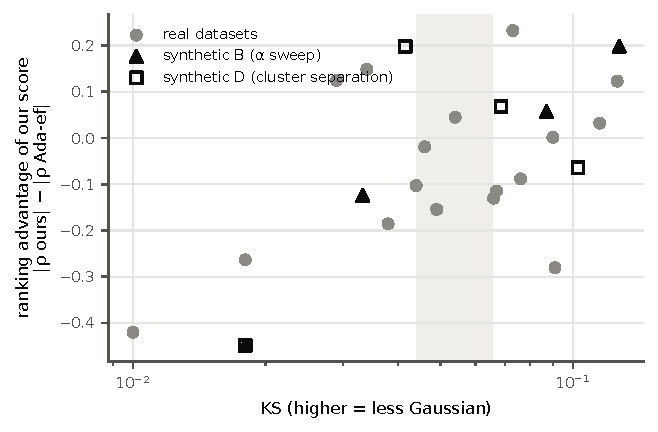
\includegraphics[width=\linewidth]{figures/fig4_controlled.pdf}
  \caption{Ranking advantage of the empirical score (its $|\rho|$ minus Ada-ef's) against KS, for the real datasets and for synthetic data with controlled anisotropy (B) and cluster
  separation (D).}
  \label{fig:controlled}
\end{figure}

\begin{figure}[h]
  \centering
  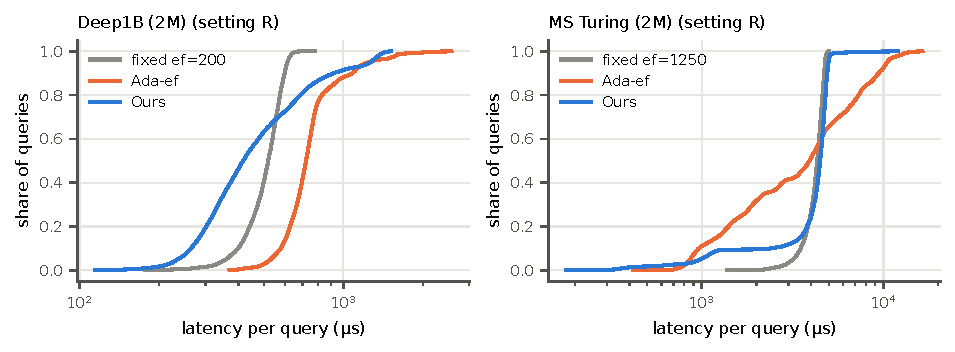
\includegraphics[width=\linewidth]{figures/fig3c_latency_cdf.pdf}
  \caption{Per-query latency on Deep1B and MS Turing (setting R). The empirical score spends less
  time on easy queries and more on hard ones; a fixed \ef{} spends about the same on all.}
  \label{fig:cdf}
\end{figure}

\begin{table*}[t]
  \caption{Time per distance computation, relative to fixed-\ef{} queries with the same distance count
  (settings P and R). Hard and easy: the 20\% of queries PercEF gives the largest and smallest \ef{},
  timed under the fixed \ef{} closest to PercEF's mean recall. Last column: PercEF's share of its
  distance computations spent on its hard queries.}
  \label{tab:querycost}
  \centering\footnotesize
  \resizebox{\linewidth}{!}{\begin{tabular}{llrrrrr}
\toprule
dataset & setting & KS & hard / fixed-ef time at same DC & easy / fixed-ef time at same DC & PercEF / fixed-ef time at same DC & PercEF DC on hard queries (\%) \\
\midrule
MS Turing (2M) & P & 0.010 & 1.009 & 1.003 & 0.991 & 95.1 \\
MS Turing (2M) & R & 0.010 & 1.003 & 0.997 & 0.981 & 97.9 \\
GloVe-100 & P & 0.018 & 1.036 & 0.803 & 1.025 & 95.7 \\
GloVe-100 & R & 0.018 & 1.036 & 0.803 & 1.014 & 97.3 \\
BIGANN (2M) & P & 0.029 & 1.076 & 0.807 & 1.032 & 50.5 \\
BIGANN (2M) & R & 0.029 & 1.087 & 0.800 & 1.025 & 39.0 \\
LAION-I2I & P & 0.034 & 1.191 & 0.842 & 1.043 & 58.0 \\
LAION-I2I & R & 0.034 & 1.174 & 0.809 & 1.057 & 54.3 \\
DBpedia-1536 & P & 0.038 & 1.048 & 0.885 & 1.000 & 81.2 \\
DBpedia-1536 & R & 0.038 & 1.057 & 0.834 & 1.036 & 66.1 \\
MS MARCO-384 & P & 0.044 & 1.132 & 0.816 & 1.004 & 30.4 \\
MS MARCO-384 & R & 0.044 & 1.134 & 0.827 & 0.971 & 30.8 \\
COCO-I2I & P & 0.046 & 1.148 & 0.925 & 1.053 & 43.8 \\
COCO-I2I & R & 0.046 & 1.168 & 0.908 & 1.051 & 35.9 \\
Cohere-1024 & P & 0.049 & 1.049 & 0.801 & 0.976 & 63.7 \\
Cohere-1024 & R & 0.049 & 1.066 & 0.837 & 1.027 & 71.2 \\
Yahoo-MiniLM & P & 0.054 & 1.084 & 0.890 & 1.022 & 44.9 \\
Yahoo-MiniLM & R & 0.054 & 1.088 & 0.893 & 1.029 & 39.8 \\
COCO-T2I & P & 0.056 & 1.005 & 1.005 & 1.011 & 100.0 \\
COCO-T2I & R & 0.056 & 1.001 & 1.001 & 1.014 & 100.0 \\
ImageNet-ALIGN & P & 0.058 & 1.009 & 1.009 & 1.031 & 100.0 \\
ImageNet-ALIGN & R & 0.058 & 1.000 & 1.000 & 1.027 & 100.0 \\
DeepImage-96 & P & 0.066 & 1.074 & 0.916 & 1.066 & 52.0 \\
DeepImage-96 & R & 0.066 & 1.089 & 0.910 & 1.076 & 43.6 \\
Deep1B (2M) & P & 0.067 & 1.092 & 0.889 & 1.053 & 34.4 \\
Deep1B (2M) & R & 0.067 & 1.084 & 0.882 & 1.074 & 43.9 \\
Fashion-MNIST & P & 0.073 & 1.093 & 0.980 & 1.017 & 30.3 \\
Fashion-MNIST & R & 0.073 & 1.091 & 0.978 & 1.015 & 25.6 \\
Landmark-DINO & P & 0.076 & 1.085 & 0.893 & 0.976 & 52.9 \\
Landmark-DINO & R & 0.076 & 1.090 & 0.892 & 0.997 & 49.0 \\
Yambda & P & 0.090 & 1.004 & 1.002 & 0.977 & 100.0 \\
Yambda & R & 0.090 & 0.999 & 0.978 & 0.989 & 100.0 \\
GIST-960 & P & 0.091 & 1.005 & 1.002 & 0.977 & 98.8 \\
GIST-960 & R & 0.091 & 1.005 & 1.002 & 0.981 & 99.4 \\
iNat-ResNet & P & 0.115 & 1.109 & 0.930 & 0.993 & 33.7 \\
iNat-ResNet & R & 0.115 & 1.123 & 0.912 & 1.000 & 30.0 \\
SIFT-1M & P & 0.126 & 1.050 & 0.896 & 1.005 & 42.7 \\
SIFT-1M & R & 0.126 & 1.060 & 0.894 & 1.006 & 28.9 \\
Last.fm & P & 0.216 & 0.999 & 0.999 & 0.985 & 100.0 \\
Last.fm & R & 0.216 & 0.996 & 0.996 & 0.994 & 100.0 \\
\bottomrule
\end{tabular}
}
\end{table*}

\begin{table*}[h]
  \caption{Offline cost.}
  \centering\footnotesize
  \begin{adjustbox}{max width=\linewidth}\begin{tabular}{llrrrrrr}
\toprule
dataset & setting & Ada-ef statistics (s) & Ada-ef table (s) & Ada-ef memory (B) & ours bins (s) & ours min-ef (s) & ours memory (B) \\
\midrule
MS Turing (2M) & P & 5.2 & 5.2 & 41,368 & 0.6 & 7.4 & 824 \\
MS Turing (2M) & R & 5.2 & 183.3 & 41,504 & 0.6 & 257.5 & 768 \\
GloVe-100 & P & -- & 36.6 & 41,392 & 0.4 & -- & 672 \\
GloVe-100 & R & -- & 370.4 & 41,608 & 0.4 & -- & 820 \\
BIGANN (2M) & P & 4.8 & 0.3 & 67,240 & 1.3 & 0.3 & 936 \\
BIGANN (2M) & R & 4.8 & 3.0 & 67,344 & 1.3 & 3.3 & 936 \\
LAION-I2I & P & -- & 21.9 & 1,053,216 & -- & -- & 2,472 \\
LAION-I2I & R & -- & 347.9 & 1,053,480 & -- & -- & 2,472 \\
DBpedia-1536 & P & -- & 1.0 & 9,450,000 & -- & -- & 6,540 \\
DBpedia-1536 & R & -- & 14.1 & 9,450,176 & -- & -- & 6,540 \\
MS MARCO-384 & P & -- & 4.5 & 593,160 & -- & -- & 1,952 \\
MS MARCO-384 & R & -- & 45.4 & 593,432 & -- & -- & 1,960 \\
COCO-I2I & P & 1.7 & 0.1 & 1,053,344 & 0.2 & 0.1 & 2,472 \\
COCO-I2I & R & 1.7 & 1.0 & 1,053,448 & 0.2 & 1.1 & 2,472 \\
Cohere-1024 & P & -- & 6.0 & 4,202,768 & -- & -- & 4,520 \\
Cohere-1024 & R & -- & 69.9 & 4,203,000 & -- & -- & 4,476 \\
Yahoo-MiniLM & P & -- & 0.3 & 593,328 & -- & -- & 1,912 \\
Yahoo-MiniLM & R & -- & 0.6 & 593,384 & -- & -- & 1,836 \\
COCO-T2I & P & 1.7 & 0.1 & 1,053,352 & 0.2 & 0.1 & 2,472 \\
COCO-T2I & R & 1.7 & 7.0 & 1,053,416 & 0.2 & 9.7 & 2,072 \\
ImageNet-ALIGN & P & -- & 0.1 & 1,643,904 & -- & -- & 2,984 \\
ImageNet-ALIGN & R & -- & 26.7 & 1,644,232 & -- & -- & 2,584 \\
DeepImage-96 & P & -- & 0.8 & 37,912 & 3.1 & -- & 808 \\
DeepImage-96 & R & -- & 9.5 & 38,192 & 3.1 & -- & 808 \\
Deep1B (2M) & P & 5.8 & 0.3 & 38,080 & 0.6 & 0.2 & 808 \\
Deep1B (2M) & R & 5.8 & 3.4 & 38,336 & 0.6 & 3.3 & 808 \\
Fashion-MNIST & P & -- & 0.1 & 2,465,040 & -- & -- & 3,560 \\
Fashion-MNIST & R & -- & 0.8 & 2,465,384 & -- & -- & 3,560 \\
Landmark-DINO & P & -- & 0.6 & 2,365,928 & -- & -- & 3,496 \\
Landmark-DINO & R & -- & 0.8 & 2,365,976 & -- & -- & 3,496 \\
Yambda & P & -- & 0.1 & 66,608 & -- & -- & 936 \\
Yambda & R & -- & 0.8 & 66,704 & -- & -- & 936 \\
GIST-960 & P & -- & 7.0 & 3,694,232 & -- & -- & 3,888 \\
GIST-960 & R & -- & 13.3 & 3,694,208 & -- & -- & 3,888 \\
iNat-ResNet & P & -- & 0.4 & 16,794,184 & -- & -- & 8,616 \\
iNat-ResNet & R & -- & 0.7 & 16,794,224 & -- & -- & 8,616 \\
SIFT-1M & P & -- & 0.1 & 66,776 & 0.4 & -- & 936 \\
SIFT-1M & R & -- & 1.4 & 67,224 & 0.4 & -- & 936 \\
Last.fm & P & 0.8 & 0.3 & 17,444 & 0.1 & 2.1 & 684 \\
Last.fm & R & 0.8 & 0.3 & 17,804 & 0.1 & 0.4 & 284 \\
\bottomrule
\end{tabular}
\end{adjustbox}
\end{table*}

\clearpage
\end{document}
